\documentclass[pmlr]{jmlr}
% OWN
\usepackage{csvsimple}
\usepackage{multirow}
\usepackage{xcolor}
\usepackage{colortbl}
\usepackage{tabu}
\usepackage[utf8]{inputenc}
\usepackage[T1]{fontenc}
\usepackage{tikz}
\usepackage{hvfloat}
\usetikzlibrary{arrows,positioning,fit,shapes,calc}

% ORIGINAL
\usepackage{rotating}% for sideways figures and tables
\usepackage{longtable}% for long tables

\usepackage{booktabs}
\usepackage[load-configurations=version-1]{siunitx} % newer version

 % The following command is just for this sample document:
\newcommand{\cs}[1]{\texttt{\char`\\#1}}

 % Define an unnumbered theorem just for this sample document:
\theorembodyfont{\upshape}
\theoremheaderfont{\scshape}
\theorempostheader{:}
\theoremsep{\newline}
\newtheorem*{note}{Note}

\usepackage[utf8]{inputenc}

 % change the arguments, as appropriate, in the following:
\jmlrvolume{1}
\jmlryear{2010}
\jmlrworkshop{Workshop Title}


% Two authors with the same address
%\author{\Name{Paweł Ksieniewicz}
%	\Email{pawel.ksieniewicz@pwr.edu.pl}\\
%	\addr 
%	Department of Systems and Computer Networks\\
%	Faculty of Electronics\\
%	Wrocław University of Science and Technology
%}
\author{\Name{--- ---}
	\Email{---}\\
	\addr 
	---\\
	---\\
	---
}

\editor{Editor's name}


\newcommand{\restable}[2] {

\scriptsize
\centering
\setlength{\tabcolsep}{3.5pt}
\def\arraystretch{1.15}
\begin{tabular}{@{}|ccccc|ccccc||ccccc|ccccc||ccc|r|}\hline%


\multicolumn{10}{|c||}{\multirow{2}{*}{\bfseries Without oversampled set}} &
\multicolumn{10}{ c||}{\multirow{2}{*}{\bfseries With oversampled set}} &
\multirow{5}{*}{\rotatebox[origin=c]{-90}{\bfseries OS}} &
\multirow{5}{*}{\rotatebox[origin=c]{-90}{\bfseries US}} &
\multirow{5}{*}{\rotatebox[origin=c]{-90}{\bfseries Full}} &
\multirow{5}{*}{\rotatebox[origin=c]{-90}{\bfseries Dataset}}
	
\\
\multicolumn{10}{|c||}{}&
\multicolumn{10}{c||}{}&
\multicolumn{3}{c|}{}&
	
	 \\
	
	\multicolumn{5}{|c|}{\bfseries Without pruning} &
	\multicolumn{5}{c||}{\bfseries With pruning} &
	\multicolumn{5}{c|}{\bfseries Without pruning} &
	\multicolumn{5}{c||}{\bfseries With pruning} 
	& & & & \\
	
	\multirow{2}{*}{\rotatebox[origin=c]{-90}{\textsc{reg}}} &
	\multirow{2}{*}{\rotatebox[origin=c]{-90}{\textsc{wei}}} &
	\multirow{2}{*}{\rotatebox[origin=c]{-90}{\textsc{con}}} &
	\multirow{2}{*}{\rotatebox[origin=c]{-90}{\textsc{nor}}} &
	\multirow{2}{*}{\rotatebox[origin=c]{-90}{\textsc{nc}}} &

	\multirow{2}{*}{\rotatebox[origin=c]{-90}{\textsc{reg}}} &
	\multirow{2}{*}{\rotatebox[origin=c]{-90}{\textsc{wei}}} &
	\multirow{2}{*}{\rotatebox[origin=c]{-90}{\textsc{con}}} &
	\multirow{2}{*}{\rotatebox[origin=c]{-90}{\textsc{nor}}} &
	\multirow{2}{*}{\rotatebox[origin=c]{-90}{\textsc{nc}}} &

	\multirow{2}{*}{\rotatebox[origin=c]{-90}{\textsc{reg}}} &
	\multirow{2}{*}{\rotatebox[origin=c]{-90}{\textsc{wei}}} &
	\multirow{2}{*}{\rotatebox[origin=c]{-90}{\textsc{con}}} &
	\multirow{2}{*}{\rotatebox[origin=c]{-90}{\textsc{nor}}} &
	\multirow{2}{*}{\rotatebox[origin=c]{-90}{\textsc{nc}}} &

	\multirow{2}{*}{\rotatebox[origin=c]{-90}{\textsc{reg}}} &
	\multirow{2}{*}{\rotatebox[origin=c]{-90}{\textsc{wei}}} &
	\multirow{2}{*}{\rotatebox[origin=c]{-90}{\textsc{con}}} &
	\multirow{2}{*}{\rotatebox[origin=c]{-90}{\textsc{nor}}} &
	\multirow{2}{*}{\rotatebox[origin=c]{-90}{\textsc{nc}}} 

	& & & &
	
	\\
	
	&&&&&&&&&&&&&&&&&&&&&&&
	\\\hline\hline
	
	\csvreader[head to column names,
	           late after line=\csvifoddrow{\\}{\\\rowcolor{gray!10!white}},
	           late after last line = \\\hline]
	{results/#1.csv}{}%
	{
	
	\ereg & \ewei & \ecwei & \enwei & \encwei &
	\eregr & \eweir & \ecweir & \enweir & \encweir &
	\eregos & \eweios & \ecweios & \enweios & \encweios & 
	\eregros & \eweiros & \ecweiros & \enweiros & \encweiros &
	\os & \us & \reg & 
	
	\multicolumn{1}{l|}{\emph{\dataset}}
	
	}%
\end{tabular}
\caption{Balanced accuracy scores obtained using #2 as a base classifier}

  
}
%TODO: Max 14 pages
%TODO: No personal information or reference to the authors should be introduced in the submitted paper.
%TODO: Submissions will be evaluated concerning their technical quality, relevance, significance, originality and clarity. 

\title
[Fusers in homogenous ensemble of undersampled majority class]
{
	Fusers in homogenous ensemble of undersampled majority class for highly imbalanced data classification%\titlebreak
}

\begin{document}

\maketitle

\begin{abstract}
This is the abstract for this article.
\end{abstract}
\begin{keywords}
classification, classifier ensemble, undersampling, imbalanced data
\end{keywords}

%%%
%%% Introduction
%%%
\section{Introduction}
\label{sec:intro}

Additionally, in incremental learning, if the majority-class objects outnumber greatly the minority class, the latter can be completely ignored \cite{He:2009}. The aforementioned issues are reasons why most existing classification methods for imbalanced data are restricted to the \textit{offline} learning only, i.e., a case where the entire data set is provided prior to the analysis.


Most of the classification algorithms assume that there are no significant disproportions among instances from different classes. Nevertheless, in many practical tasks, we may observe that instances from one class (so-called \textit{majority class}) significantly outnumber the objects from remaining classes (\textit{minority class}). Most of traditional classifiers have a bias in favor of the majority class although more often the minority class is more interesting, because misidentification of an instance belonging to it is usually much more expensive than assigning an instance from majority class to minority one. A good example is an undetected fraud that would be more expensive than the cost of additional analysis of a correct transaction classified as fraudless transaction. Such a problem is known as imbalanced data classification \cite{Sun:2009,Wang:2017}, where an unequal number of instances from the examined classes plays a key role during the classifier learning. Various approaches have been proposed in the literature to tackle this challenging difficulty embedded in the nature of data. Usually, the researchers are focusing on maximizing the correct minority class classification. At the same time, performance on the majority class cannot be neglected.

\begin{figure}[!h]
\floatconts
  {fig:east}
  {\caption{Easy separable imbalance dataset}}
  {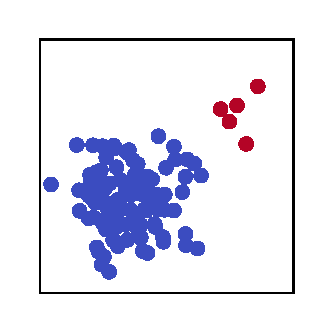
\includegraphics[clip=true, trim = 11 11 11 11, width=0.25\linewidth]{figures/easy}}
\end{figure}

In this project we will focus on binary imbalanced problems, because this setup is the one most frequently studied in the literature and most commonly meet in practical problems, e.g.,\textit{fault detection} or \textit{spam filtering}. Therefore, another important issue is proposing an appropriate quality measure that would be adequate for imbalanced data classification \cite{Elazmeh:2006}.

In case of imbalanced data classification the disproportion between the different classes is not the sole issue of learning difficulties. One may easily came up with an example where the instance distributions from different classes are well-separated, as depicted in Fig.\ref{fig:easy}.

Proposing a efficient classifier for such a task is not a challenge. Unfortunately, instances from the minority class often form clusters of an unknown structure that are scattered \cite{Napierala:2012}. Additional complication comes from the fact that during learning, the number of intactness from the minority class may be not sufficient enough for the learning algorithm to acquire the appropriate generalization level, which in effect can cause \emph{overfitting} \cite{Chen:2008}. All those problems are a focus of intense research \cite{Chawla:2002,Bunkhumpornpat:2009,Kubat:1997}.

Methods for imbalanced data classification can be divided into three main groups \cite{Lopez:2012}.

\begin{figure}[!h]
\floatconts
  {fig:subfigex}
  {\caption{Examples of data preprocessing methods.}}
  {%
    \subfigure[Original dataset]{\label{fig:circle}%
    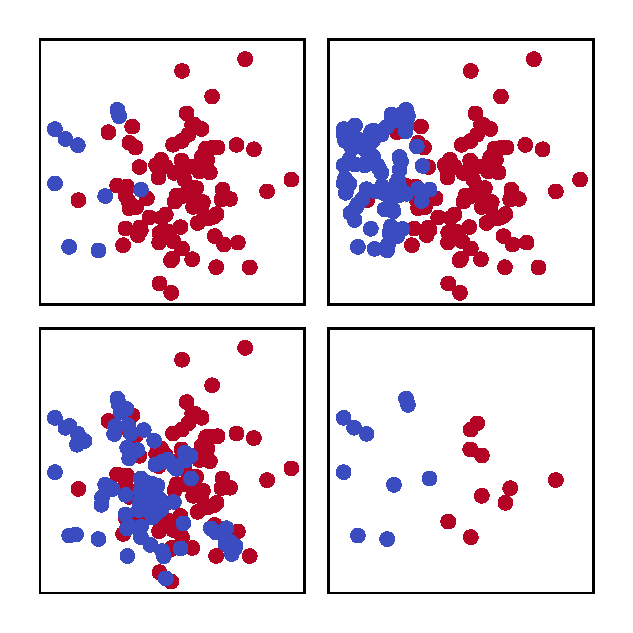
\includegraphics[clip=true, width=.25\linewidth,
    				 trim = 11 141 141 11]
    {figures/preprocessing}}%
    \qquad
    \subfigure[\textsc{smote}]{\label{fig:circle}%
    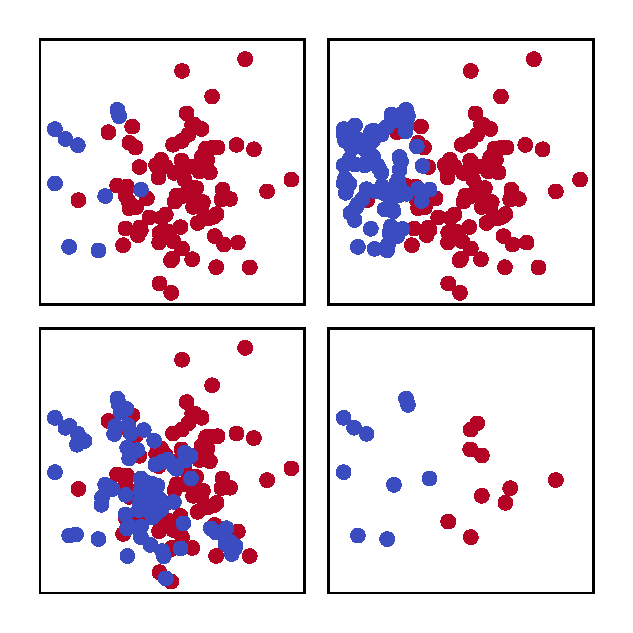
\includegraphics[clip=true, width=.25\linewidth,
    				 trim = 141 141 11 11]
    {figures/preprocessing}}%
       
    \subfigure[\textsc{adasyn}]{\label{fig:circle}%
    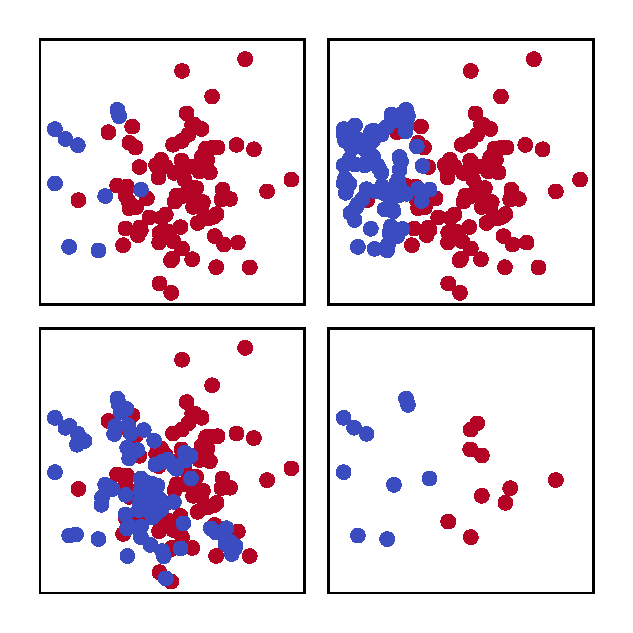
\includegraphics[clip=true, width=.25\linewidth,
    				 trim = 11 11 141 141]
    {figures/preprocessing}}%
    \qquad
    \subfigure[Undersampling]{\label{fig:circle}%
    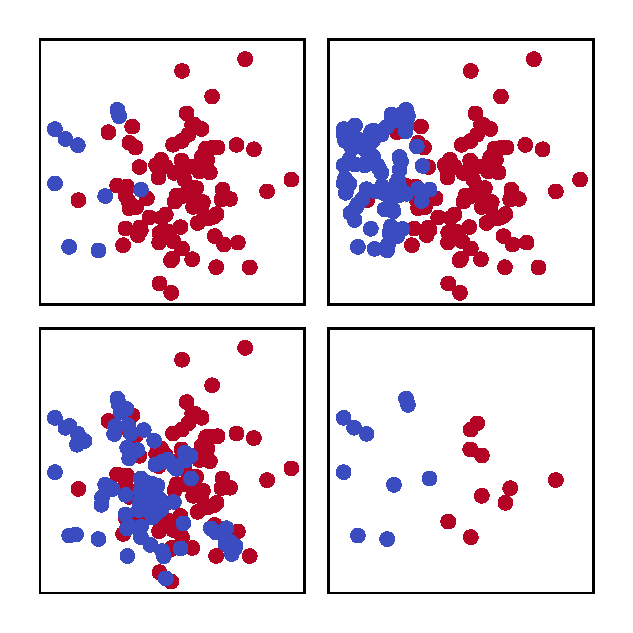
\includegraphics[clip=true, width=.25\linewidth,
    				 trim = 141 11 11 141]
    {figures/preprocessing}}%
  }
\end{figure}

\noindent\textbf{ Data preprocessing methods}. This approach focuses on reducing the number of objects in majority class (\emph{undersampling}) or generating new objects of the minority class (\textit{oversampling}). The difference between \emph{under-} and \emph{oversampling} is presented in Fig. \ref{fig:over-under}.

These mechanisms have the objective of balancing the quantity of instances from considered classes. For oversampling, new instances are random copies of existing ones or are generated in a guided manner. The most popular method is \textsc{smote} \cite{Cha2002} algorithm, which creates new instances on a basis of existing ones by slightly modifying the values of their attributes. As a result, new artificial examples that are in compliance with the minority class distribution are generated.  Other oversampling methods are \textsc{adasyn} \cite{He:2008}, in which a difficulty of an object for the classifying model is considered or \textsc{ramob}oost \cite{Chen:2010}. Unfortunately, methods such as \textsc{smote} may lead to changes in the characteristic of the minority class and in result to \emph{overfitting} the classifier, what was shown in Fig. \ref{fig:wrong_smote}.

\begin{figure}[htbp]
\floatconts
  {fig:subfigex}
  {\caption{Example of wrong \textsc{smote} oversampling.}}
  {%
    \subfigure[Original dataset]{\label{fig:circle}%
    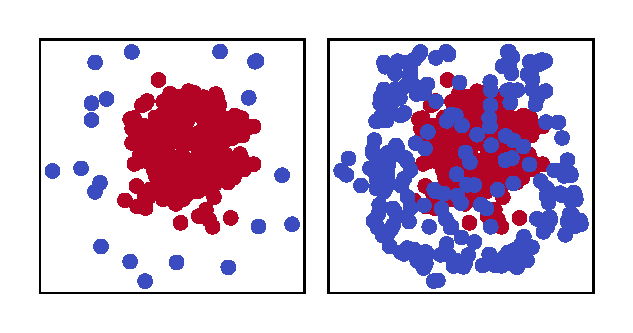
\includegraphics[clip=true, width=.25\linewidth,
    				 trim = 11 11 141 11]
    {figures/wrong_smote}}%
    \qquad
    \subfigure[\textsc{smote}]{\label{fig:circle}%
    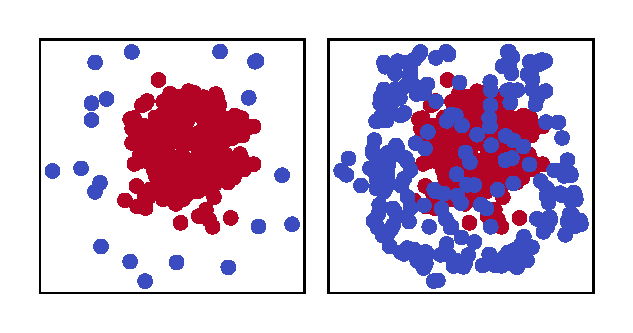
\includegraphics[clip=true, width=.25\linewidth,
    				 trim = 141 11 11 11]
    {figures/wrong_smote}}%
  }
\end{figure}

W WYPADKU UNDERSAMPLINGU NIE WYSTEPUJE RYZYKO NIESŁUSZNEGO ROZSZERZENIA PRZESTRZENI WZORCÓW KLASY MNIEJSZOŚCIOWEJ, CO MA MIEJSCE W CHOĆBY SMOTE.


Several modifications of \textsc{smote} have been proposed that are able to identify the instances to be copied in a more intelligent fashion such as \emph{Borderline}\textsc{smote} \cite{Han:2005}. It generates new instances from the minority class close to the decision border. \emph{Safe-Level} \textsc{smote} \citep{Bunkhumpornpat:2009} and \textsc{ln}-\textsc{smote} \cite{Maciejewski:2011} reduce the probability of generating synthetic instances of the minority class in areas where the predominant objects are that of the majority class. It is worth noticing that our team proposed two novel solutions to this problem: \textsc{rbo} \cite{koziarski2017radial} and \textsc{ccr} that enforce instances from the majority-class to be relocated from the areas where the minority-class instances are present \cite{Koziarski:2017amcs}. Methods of \emph{undersampling} are built around the idea of randomly removing the instances from the majority-class or removing them from the areas in such way that the  quality of the classifier is not disrupted using neighbor analysis.%\todo{W opisie metod przetwarzania wstępnego skupiamy się chyba wyłącznie na \emph{oversamplingu}.}\todo{Nie uwzględniłem czystego losowego \emph{oversamplingu}, bo skoro powtarza istniejące już obiekty, to ilustracja byłaby bezsensowna.}

%\begin{figure}[hbt]
%\centering
%\includegraphics[width=.9\linewidth]{figures/smote}
%\caption{Example of oversampling using \textsc{smote}}
%\end{figure}

\noindent\textbf{ Inbuilt mechanisms.} In this approach existing classification algorithms are adapted for imbalanced problems ensuring balanced accuracy for instances from both classes. Two of the most popular areas of research of this methods are using one-class classification  \cite{Japkowicz:1995}, usually known as learning without counterexamples, where the goal is to learn the minority class decision areas and because of the frequently assumed regular, closed shape of the decision borders is adequate to the clusters created by minority classes \cite{Krawczyk:2014ins}. The disproportion between the number of instances in classes is then omitted. Another approach is the (\textit{cost sensitive}) classification, where the algorithm takes into account the asymmetrical loss function that assigns a higher cost to a misclassification of an instance form a minority class \cite{Krawczyk:2014,Lopez:2012,He:2009,Zhou:2006}. Unfortunately such methods can cause a reverse bias towards the minority class. 
Worth noting are methods based on ensemble classification \cite{Wozniak:2014}, like \emph{\textsc{smote}Boost} \cite{Chawla:2003} and \emph{AdaBoost.NC} \cite{Wang:2010}%, or \emph{Multi-objective Genetic Programing Ensemble} \cite{Bhowan:2013}.


\noindent\textbf{Hybrid methods.} They combine the advantages of methods using data pre-processing with the classification methods. The most popular category is the hybridisation of \emph{under-} and \emph{oversampling} with ensemble classifiers \cite{Galar:2012}. This approach allows the data to be independently  processed for each of the base model. Algorithms formed on modifications of \emph{Bagging} and \emph{Boosting} \cite{Chawla:2003} enjoy wide popularity.

The main contributions of this work are:

%%%
%%% Introduction
%%%
\section{Homogenous ensemble based on undersampling the majority class}
\label{sec:intro}

Zaawansowane metody oversamplingu nie są możliwe do zastosowania przy sytuacji, gdzie w zbiorze uczącym znajduje się zaledwie kilka wzorców.

Idea k-foldowego podziału klasy większościowej. Wyznaczanie wartości k jako zaokrąglonego IR. Atut w postaci wykorzystania wszystkich wzorców, gdzie tworzymy komitet k zbalansowanych zbiorów.

\begin{figure}[htbp]
\floatconts
  {fig:teximage}
  {\caption{Scheme of using k-Fold division in ensemble construction}}
  {\includeteximage[angle=0]{figures/ensemble_scheme}}
\end{figure}

Wyliczanie wag. Accuracy się nie sprawdzi, więc BAC.

Jeśli klasyfikujemy nie jeden wzorzec, a wiele, wagi mogą być też dla pojedynczych próbek, dla podbicia, a więc pojawia się KONTRAST. Mamy takie ładne ilustracje z badań, dodajmy rysunek chociaż jeden poglądowo.

\begin{figure}[!h]
\floatconts
  {fig:subfigex}
  {\caption{Rysunek.}}
  {%
    \subfigure[O jaki ładny]{\label{fig:circle}%
    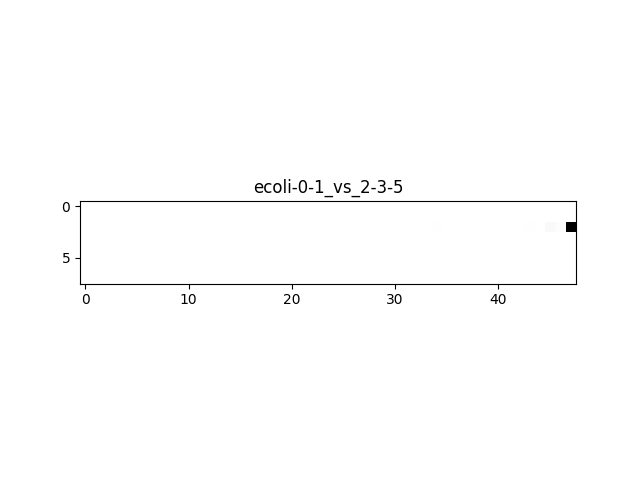
\includegraphics[width=.5\linewidth, trim = 0 100 0 100,clip=true]
    {figures/ecoli-0-1_vs_2-3-5}}%
    \subfigure[A ten brzydki]{\label{fig:circle}%
    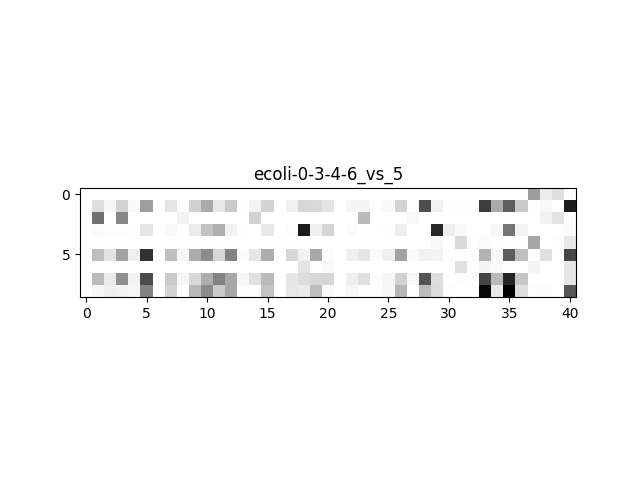
\includegraphics[width=.5\linewidth, trim = 0 100 0 100,clip=true]
    {figures/ecoli-0-3-4-6_vs_5}}%
  }
\end{figure}

Potencjał kontrastu dla danych strumieniowych.

Proponowane metody decyzyjne.

\begin{itemize}
	\item - akumulacja wsparć,
	\item - akumulacja ważona po członkach komitetu, gdzie waga to BAC dla zbioru uczącego,
	\item - akumulacja ważona po wzorcach, przez kontrast,
	\item - akumulacja znormalizowanych wag członków,
	\item - iloczyn znormalizowanych wag i kontrastu
\end{itemize}

Duża skala niezbalansowania to duża wielkość komitetu (ilustracja zależności na wykresie). Przyda się więc przycinanie (pruning).

Wyjaśnienie podejścia do pruningu. Wyliczamy wzajemną zależność statystyczną (Wilcoxonem) pomiędzy wsparciami członków i grupujemy -- omijając kwestię 1z2 2z3 ale nie 1z3 -- je uśredniając wsparcia w obrębie grupy. Uśredniamy też wagi i tworzymy tak dwupoziomowy system fuzji (potrzebna ilustracja).

Pruning też jest w kontekście klasyfikacji wielu wzorców na raz.

Wyjaśnienie kwestii wspomnianej wcześniej i uzasadnienie pominięcia jej analizy. 

%%%
%%% Introduction
%%%
\section{Experiment design}
\label{sec:intro}

Wybrane zbiory danych.

Wykorzystane klasyfikatory bazowe. Wyjaśnienie dlaczego odrzuciliśmy MLP (brak konwergencji na bardzo niewielkich zbiorach) i SVC (nie jest on naturalnie probabilistyczny, a jego probabilistyczna interpretacja jest silnie zakłamana przy niewielkich zbiorach danych). Stąd bierzemy GNB, kNN i DT, przy domyślnych parametrach z sklearn.

Powównawczo uczenie na pełnym zbiorze i zbiorach po pojedynczym under i oversamplingu.

Undersampling, ze względu na niestabilność, powtórzony pięciokrotnie na każdym foldzie.

Zastosowana metoda podziału -- wymuszone przez KEEL k-fold CV (z k=5). 

Zastosowana miara jakości -- zbalansowana dokładność, wymierna w niezbalansowanych danych.

Zastosowana analiza statystyczna -- parowa zależność pomiędzy klasyfikatorem z najwyższym rezultatem a pozostałymi w postaci testu Wilcoxona.

Przygotowane oprogramowanie ze wskazaniem repozytorium.

%%%
%%% Introduction
%%%
\section{Experimental evaluation}
\label{sec:intro}

Przedstawienie tabel.

\begin{sidewaystable}
	\restable{GNB}{\textsc{gnb}}
\end{sidewaystable}

\begin{sidewaystable}
	\restable{kNN}{k\textsc{nn}}
\end{sidewaystable}

\begin{sidewaystable}
	\restable{DTC}{\textsc{dtc}}
\end{sidewaystable}

Tabela zbiorcza zwycięstw w zależności od parametrów (z grupowaniem).

Interpretacja wyników, czyli co zostało należycie uprawdopodobnione.

%%%
%%% Conclusions
%%%
\section{Conclusions}
\label{sec:intro}
Co zostało zaproponowane.

Na co pozwala taka metoda.

Do jakich rezultatów doprowadziła.

Jakie są plany na przyszłość (czyli co robisz w wakacje).



%%%
%%% Acknowledgements and references
%%%
\acks{
	Acknowledgements go here.
}
\bibliography{bibliography}

\end{document}
